\tikzset{>=latex} % for LaTeX arrow head
\contourlength{1.2pt}

\colorlet{myred}{red!65!black}
\tikzstyle{ground}=[preaction={fill,top color=black!10,bottom color=black!5,shading angle=20},
                    fill,pattern=north east lines,draw=none,minimum width=0.3,minimum height=0.6]
\tikzstyle{mass}=[line width=0.6,red!30!black,fill=red!40!black!10,rounded corners=1,
                  top color=red!40!black!20,bottom color=red!40!black!10,shading angle=20]
\tikzstyle{rope}=[brown!70!black,line width=1.2,line cap=round] %very thick

\tikzstyle{force}=[->,myred,thick,line cap=round]
\tikzstyle{Fproj}=[force,myred!40]
\newcommand{\vbF}{\vb{F}}
\newboolean{showforces}
\setboolean{showforces}{true}

% HORIZONTAL ground
\def\h{0.7} % mass height
\def\w{0.9} % mass width




% FRICTION static/dynamical


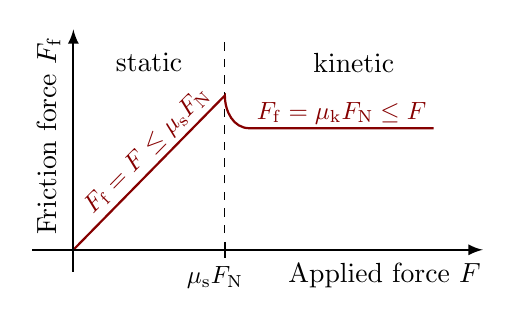
\begin{tikzpicture}
  \def\xmax{5.2}
  \def\ymax{2.8}
  \def\xc{0.37*\xmax}
  \def\yc{0.7*\ymax}
  \draw[dashed] (\xc,0) --++ (0,0.97*\ymax); % coordinate (C);
  \draw[myred!80!black,thick]
    (0,0) -- (\xc,\yc)
    node[scale=0.9,midway,right=5,above=3,rotate={atan2(\yc,\xc)}] {$F_\mathrm{f} = F \leq \mu_\mathrm{s}F_\mathrm{N}$}
    to[out=-90,in=180]++ (0.06*\xmax,-0.08*\xmax) --++ (0.45*\xmax,0)
    node[scale=0.9,midway,above=-2] {$F_\mathrm{f} = \mu_\mathrm{k}F_\mathrm{N} \leq F$};
  \draw[->,thick] (-0.1*\xmax,0) -- (\xmax,0) node[right=4,below left=1] {Applied force $F$};
  \draw[->,thick] (0,-0.1*\ymax) -- (0,\ymax) node[above left=1,rotate=90] {Friction force $F_\mathrm{f}$};
  \draw[thick] (\xc,0.1) --++ (0,-0.2) node[scale=0.9,left=4,below] {$\mu_\mathrm{s}F_\mathrm{N}$};
  \node[] at (\xc/2,0.85*\ymax) {static};
  \node[] at ({(\xmax+\xc)/2},0.85*\ymax) {kinetic};
  
\end{tikzpicture}
